%% Преамбула TeX-файла

% 1. Стиль и язык
\documentclass[utf8x]{G7-32} % Стиль (по умолчанию будет 14pt)
\usepackage[T2A]{fontenc}
\usepackage[russian]{babel}
\usepackage{verbatim}
% Остальные стандартные настройки убраны в preamble.inc.tex.
\sloppy

% Настройки стиля ГОСТ 7-32
% Для начала определяем, хотим мы или нет, чтобы рисунки и таблицы нумеровались в пределах раздела, или нам нужна сквозная нумерация.
\EqInChapter % формулы будут нумероваться в пределах раздела
\TableInChapter % таблицы будут нумероваться в пределах раздела
\PicInChapter % рисунки будут нумероваться в пределах раздела

% Добавляем гипертекстовое оглавление в PDF
\usepackage[
bookmarks=true, colorlinks=true, unicode=true,
urlcolor=black,linkcolor=black, anchorcolor=black,
citecolor=black, menucolor=black, filecolor=black,
]{hyperref}

% Изменение начертания шрифта --- после чего выглядит таймсоподобно.
% apt-get install scalable-cyrfonts-tex

\IfFileExists{cyrtimes.sty}
    {
        \usepackage{cyrtimespatched}
    }
    {
        % А если Times нету, то будет CM...
    }

\usepackage{graphicx}   % Пакет для включения рисунков

% С такими оно полями оно работает по-умолчанию:
% \RequirePackage[left=20mm,right=10mm,top=20mm,bottom=20mm,headsep=0pt]{geometry}
% Если вас тошнит от поля в 10мм --- увеличивайте до 20-ти, ну и про переплёт не забывайте:
\geometry{right=20mm}
\geometry{left=30mm}


% Пакет Tikz
\usepackage{tikz}
\usetikzlibrary{arrows,positioning,shadows}

% Произвольная нумерация списков.
\usepackage{enumerate}

% ячейки в несколько строчек
\usepackage{multirow}

% itemize внутри tabular
\usepackage{paralist,array}


% Настройки листингов.
% 8 Листинги

\usepackage{listings}

% Значения по умолчанию
\lstset{
  basicstyle= \footnotesize,
  breakatwhitespace=true,% разрыв строк только на whitespacce
  breaklines=true,       % переносить длинные строки
%   captionpos=b,          % подписи снизу -- вроде не надо
  inputencoding=koi8-r,
  numbers=left,          % нумерация слева
  numberstyle=\footnotesize,
  showspaces=false,      % показывать пробелы подчеркиваниями -- идиотизм 70-х годов
  showstringspaces=false,
  showtabs=false,        % и табы тоже
  stepnumber=1,
  tabsize=4,              % кому нужны табы по 8 символов?
  frame=single
}

% Стиль для псевдокода: строчки обычно короткие, поэтому размер шрифта побольше
\lstdefinestyle{pseudocode}{
  basicstyle=\small,
  keywordstyle=\color{black}\bfseries\underbar,
  language=Pseudocode,
  numberstyle=\footnotesize,
  commentstyle=\footnotesize\it
}

% Стиль для обычного кода: маленький шрифт
\lstdefinestyle{realcode}{
  basicstyle=\scriptsize,
  numberstyle=\footnotesize
}

% Стиль для коротких кусков обычного кода: средний шрифт
\lstdefinestyle{simplecode}{
  basicstyle=\footnotesize,
  numberstyle=\footnotesize
}

% Стиль для BNF
\lstdefinestyle{grammar}{
  basicstyle=\footnotesize,
  numberstyle=\footnotesize,
  stringstyle=\bfseries\ttfamily,
  language=BNF
}

% Определим свой язык для написания псевдокодов на основе Python
\lstdefinelanguage[]{Pseudocode}[]{Python}{
  morekeywords={each,empty,wait,do},% ключевые слова добавлять сюда
  morecomment=[s]{\{}{\}},% комменты {а-ля Pascal} смотрятся нагляднее
  literate=% а сюда добавлять операторы, которые хотите отображать как мат. символы
    {->}{\ensuremath{$\rightarrow$}~}2%
    {<-}{\ensuremath{$\leftarrow$}~}2%
    {:=}{\ensuremath{$\leftarrow$}~}2%
    {<--}{\ensuremath{$\Longleftarrow$}~}2%
}[keywords,comments]

% Свой язык для задания грамматик в BNF
\lstdefinelanguage[]{BNF}[]{}{
  morekeywords={},
  morecomment=[s]{@}{@},
  morestring=[b]",%
  literate=%
    {->}{\ensuremath{$\rightarrow$}~}2%
    {*}{\ensuremath{$^*$}~}2%
    {+}{\ensuremath{$^+$}~}2%
    {|}{\ensuremath{$|$}~}2%
}[keywords,comments,strings]

% Подписи к листингам на русском языке.
\renewcommand\lstlistingname{\cyr\CYRL\cyri\cyrs\cyrt\cyri\cyrn\cyrg}
\renewcommand\lstlistlistingname{\cyr\CYRL\cyri\cyrs\cyrt\cyri\cyrn\cyrg\cyri}


% Полезные макросы листингов.
% Любимые команды
\newcommand{\Code}[1]{\textbf{#1}}


\begin{document}

\pagestyle{empty}
\begin{center}
    Министерство образования и науки Российской Федерации\\
    ФГАОУ ВПО  «УрФУ имени первого Президента России Б. Н. Ельцина»\\
    Институт радиоэлектроники и информационных технологий - РтФ\\
    Департамент информационных технологий и автоматики
    \par
    \vspace{4.5cm}
    \Large{
      Иммитационное моделирование в  системе Bizagi Proces Modeler

      \par
      \vspace{0.5cm}

      ОТЧЕТ\\
      по лабораторной работе
    }

    \vspace{4cm}
    {
      Преподаватель: \hfill Клебанов Борис Исаевич
    }
    \par
    {
      Студент: \hfill Сухоплюев Илья Владимирович
    }
    \par
    {
      Группа: \hfill РИ-440001
    }

    \par
    \vspace{3.5cm}
    Екатеринбург\\
    2017
\end{center}


\frontmatter % выключает нумерацию ВСЕГО; здесь начинаются ненумерованные главы: реферат, введение, глоссарий, сокращения и прочее.

% Команды \breakingbeforechapters и \nonbreakingbeforechapters
% управляют разрывом страницы перед главами.
% По-умолчанию страница разрывается.

% \nobreakingbeforechapters
% \breakingbeforechapters

% % Также можно использовать \Referat, как в оригинале
\begin{abstract}
Это пример каркаса расчётно-пояснительной записки, желательный к использованию в РПЗ проекта по курсу РСОИ.

Данный опус, как и более новые версии этого документа, можно взять по адресу (\url{https://github.com/rominf/latex-g7-32}).

Текст в документе носит совершенно абстрактный характер.
\end{abstract}

%%% Local Variables: 
%%% mode: latex
%%% TeX-master: "rpz"
%%% End: 

\pagestyle{plain}

\tableofcontents

% \Defines % Необходимые определения. Вряд ли понадобться
\begin{description}
\item[Распределённый] Слово, которое нельзя употреблять. Но надо протестировать длинные строки в глоссарии.
\end{description}

%%% Local Variables:
%%% mode: latex
%%% TeX-master: "rpz"
%%% End:

% \Abbreviations %% Список обозначений и сокращений в тексте
\begin{description}
\item[АИС] Автоматизированная информационная система. Но надо протестировать длинные строки в определениях.
\end{description}

%%% Local Variables:
%%% mode: latex
%%% TeX-master: "rpz"
%%% End:


\Introduction

Целью работы является создание всякой всячины. Для достижения поставленной цели необходимо решить следующие задачи:

\begin{itemize}
\item проанализировать существующую всячину;
\item спроектировать свою, новую всячину;
\item изготовить всякую всячину;
\item проверить её работоспособность.
\end{itemize}

Вот так-то. А этот абзац вставлен для визуальной оценки отступа от перечня до следующего абзаца.

\mainmatter % это включает нумерацию глав и секций в документе ниже

\chapter{Исспользуемые технологии}\label{technologies}

В данной разделе рассматриваются используемые программы и технологии,
используемые в данной работе и цель их использования.

\section{Kernel-based Virtual Machine (KVM) и libvirt}

Кластерная система -- это группа компьютеров, объединенных высокоскоростными
каналами связи, которая будет представлять для пользователя единый аппаратный
ресурс.

Для того, чтобы полноценно протестировать установку и настройку такой системы,
нам потребовалось несколько компьютеров и коммутатор(-ов) соединяющих их между
собой, что не очень целесообразно для тестовой задачи. Для этого в настоящий
момент времени удобно создавать такие системы с использованием виртуальных
машин и виртуальных сетей, которые будут эмулировать поведение реального
оборудования.

В Ubuntu рекомендуется использовать гипервизор (менеджер виртуальных машин)
\textmd{KVM}\cite{kvm} и библиотеку \textmd{libvirt}\cite{libvirt} в качестве инструментария
управления им.

\myImage{Virt-manager -- GUI-интерфейс для управления виртуальными машинами}{virt-manager}{virt-manager}

Также для простоты использования к данным инструментам можно поставить
\textmd{virt-manager}(Рис. \ref{virt-manager}) -- GUI-интерфейс, позволяющий
легко создавать виртуальные машины и управлять ими.

\section{Операционная система -- CentOS7}

Каждый узел (или нода) в нашей кластерной системе будет представлять
отдельный компьютер с установленной системой \textmd{CentOS7}\cite{centos},
основанной на пакетном менеджере \textmd{yum} и впервые выпущенной 14 мая 2004 года.
Эта операционная система основана на коммерческом проекте
\textmd{Red Hat Enterprise Linux}\cite{rhel} и совместима с ним.

Данная операционная система позволяет автоматизировать установку с помощью
\textmd{kickstart}-файла\cite{rhel-kickstart}, описывающего выбор вариантов,
которые предлагаются перед установкой системы.

\section{Network File System (NFS)}

Network File System (NFS) — протокол сетевого доступа к файловым системам,
первоначально разработан Sun Microsystems в 1984 году. За основу был взят протокол
вызова удалённых процедур (RPC). Позволяет подключать (монтировать) удалённые
файловые системы через сеть.

В нашей задаче данная технология потребуется для запуска MPI-программ, которые
подразумевают что запускаемая программа доступна на всех узлах системы.
Конечно, для этих целей можно просто провести копирование исполняемого файла
на все узлы, но постоянная работа таким образом является утомительной, что
в конечном итоге повлечет за собой создание скрипта или другого механизма
по автоматизации этого процесса. Чтобы избежать этого мы создадим каталог,
доступный через с помощью NFS всем узлам.

\section{MPI (Intel MPI)}

\textmd{Message Passing Interface} (MPI, интерфейс передачи сообщений) -- стандарт
программного интерфейса (API) для передачи информации, который позволяет
обмениваться сообщениями между процессами, выполняющими одну задачу.
Разработан Уильямом Гроуппом, Эвином Ласком (англ.) и другими\cite{mpi}.

Существует множество реализаций MPI. В данной работе мы будем разворачивать
\textmd{Intel MPI}\cite{intel-mpi}, в предположении что эта реализация
наибыстрейшая.

\section{Архитектура кластера}

Обсудим общую схему создаваемой системы. Краткое описание можно увидеть на
рисунке \ref{arch}. В текущем примере мы будем создавать кластер из 3-х узлов,
представляющих виртуальные машины с \textmd{CentOS7}, соединенных двумя сетями.

Первая сеть будет необходима для доступа в сеть Интернет и скачивания
требуемых rpm-пакетов. Вторая сеть будет использоваться для взаимодействия между
узлами и будет изолированной, поскольку протокол NFS подразумевает подключение
по доверенной сети.

Конфигурация первой сети:
\begin{verbatim}
  IP-пространство: 192.168.127.0/24
  Шлюз по-умолчанию: 192.168.127.1 (Рабочая станция, NAT до Интернета)
  DHCP-pool: 192.168.127.128 - 192.168.127.254
\end{verbatim}

Конфигурация второй сети:
\begin{verbatim}
  статическое IP-пространство: 10.20.30.0/24
\end{verbatim}

\clearpage

\myImage{Общая схема разворачиваемой системы}{arch}{arch}
Все узлы будут иметь названия хоста (node1/node2/node3). node1-узел
будет главным, а также будет размещать на себе NFS-сервер и предоставлять
папку /nfs двум другим узлам, которые будут NFS-клиентами.

Для того, чтобы обеспечить автоматическую установку системы
\textmd{CentOS}, потребуется обеспечить доступ к kickstart-файлам, которые
будут сгенерированны для каждого компьютера и располагаться на локальном
HTTP-сервере. Там же будет располагаться архив mpi.tgz с Intel MPI-установочником,
который будет установлен после основной установки системы.

\chapter{Создание кластерной системы}

В этой главе рассматриваются пошаговые действия при подготовке
автоматизированной установки кластерной системы из 3-ех нод,
описанной в предыдущей главе.

\section{Создание виртуальных сетей}

Для создания новой виртуальной сети в \textmd{virt-manager}
перейдем в "Правка"$\rightarrow$"Свойства подключения"$\rightarrow$"Виртуальные сети"
и в открывшемся диалоговом окне найдем кнопку по созданию сети.
Конфигурации сетей изображены на Рис. \ref{network-mpi} и
\ref{network-mpi-offline}.

\myImage{Конфигурация первой сети для доступа в Интернет}{network-mpi}{network-mpi}
\myImage{Конфигурация второй, внутренней сети}{network-mpi-offline}{network-mpi-offline}

\clearpage

\section{Получение основного kickstart-файла}

Следующим шагом, мы должны создать kickstart-файл, где будут
описаны все основные этапы установки системы. Kickstart-файл
представляет из себя простой текстовый файл (plain text)
который разбит на обязательные и опциональные секции. Создание
и отладка такого файла -- довольно трудоемкая задача. Для
упрощения его получения, можно провести тестовую установку
системы, после чего в домашней папке пользователя \textmd{root}
будет лежать файл \textmd{anaconda-ks.cfg}, сохронивший в
себе все этапы выбора при установке.

\myImage{Добавление второго сетевого интерфейса}{centos-vm}{centos-vm}

Для этого выберем пункт "Создать виртуальную машину" и
проследуем мастеру настройки, указав скаченный с официального сайта
образ CentOS и созданную сеть с доступом в Интернет. Также выберем пункт
"Дополнить конфигурацию перед установкой", чтобы добавить
второй интерфейс к доступу в изолированную сетью (Рис\ref{centos-vm}),
модель интерфейсов \textmd{virtio}, а для ускорения установки
в параметрах жесткого диска можно указать "unsafe" - кэширования.
\clearpage

\myImage{Процесс установки CentOS7}{centos-install}{centos-install}

После настройки физической конфигурации машины, мы можем нажать
"Начать установку" и перед нами раскроется окно с эмуляцией
монитора созданной машины. В ней мы увидим приглашение к установке
CentOS7, в которой можем произвести всю необходимую настройку
(Рис. \ref{centos-install}). После того, как мы
нажмем "Начать установку", мы сможем настроить пользователей
системы.

Наконец, перезагрузив систему и зайдя от \textmd{root}-пользователя
мы найдем файл \textmd{anaconda-ks.cfg}. При желании полученный
файл можно найти в приложении \ref{app:kickstart}.

\clearpage

\section{Генерация kickstart-файла с помощью python}
Для установки нескольких узлов, нам потребуется создать
копии полученного \textmd{kickstart}-файла. При этом
данные файлы будут отличаться только именем узла и
статическим IP-адрессом в изолированной сети. Мы можем
создать из полученного файла Jinja-шаблон\cite{jinja2}, и
сгенерировать полученные конфиги автоматически, в зависимости
от номера узла:

\verbatiminput{listings/generate.py}

А в шаблоне заменить изменяющиеся параметры:

\begin{verbatim}
# ...

network  --bootproto=static --device=eth1 --ip={{ip}} \
           --netmask=255.255.255.0 --ipv6=auto --activate
network  --hostname={{host}}

# ...
\end{verbatim}

После чего мы можем просто раздать http-сервером эти файлы.
И при установке дописав параметр, который запустит
автоматическую установку:
\begin{verbatim}
  inst.ks=http://192.168.127.1:8080/node1.cfg
\end{verbatim}

\section{Настройка NFS}

Рассмотрим настройку NFS-подсистемы, которая сделает общий
подкаталог \textmd{/nfs} для всех узлов. Данный критерий не
обязателен при работе с MPI, но очень упрощает разработку.

\subsection{Настройка NFS-сервера}

Для настройки nfs в CentOS есть пакеты \textmd{nfs-utils} и
\textmd{nfs-utils-lib}. В процессе установки
использовался DVD-образ CentOS7, и эти пакеты были выбраны
при установке. Поэтому остается только провести настройку
узлов:
\begin{verbatim}
mkdir -p /nfs # создадим общую
vim /etc/exports # правим конфигурацию nfs-сервера
\end{verbatim}
В /etc/exports вписываем следующую строку:
\begin{verbatim}
/nfs 10.20.30.0/24(rw,sync,no_root_squash,no_all_squash)
\end{verbatim}
При этом:
\begin{itemize}
  \item /home/nfs – расшариваемая директория;
  \item 10.20.30.40/24 – IP адрес клиента (или, как в моем случае, возможность подключения для всей подсети);
  \item rw – разрешение на запись;
  \item sync – синхронизация указанной директории;
  \item no\_root\_squash – включение root привилегий;
  \item no\_all\_squash — включение пользовательской авторизации;
\end{itemize}
После чего включаем все необходимые сервисы:
\begin{verbatim}
systemctl enable rpcbind
systemctl enable nfs-server
systemctl enable nfs-lock
systemctl enable nfs-idmap
systemctl start rpcbind
systemctl start nfs-server
systemctl start nfs-lock
systemctl start nfs-idmap
\end{verbatim}

\subsection{Настройка NFS-клиента}

Со стороны клиента требуется гораздо меньше забот. Достаточно
включить необобходимые сервисы:
\begin{verbatim}
systemctl enable rpcbind
systemctl enable nfs-server
systemctl enable nfs-lock
systemctl enable nfs-idmap
systemctl start rpcbind
systemctl start nfs-server
systemctl start nfs-lock
systemctl start nfs-idmap
\end{verbatim}
И примонтировать папку с сервера:
\begin{verbatim}
mkdir -p /nfs
mount -t nfs 10.20.30.41:/nfs /nfs
\end{verbatim}
После чего можно проверить работоспособность:
\begin{verbatim}
echo "Hello, NFS!" > /nfs/hello
# на node1 должен появится файл /nfs/hello
\end{verbatim}
И наконец, чтобы не монтировать NFS при каждом запуске,
подправим файл \textmd{/etc/nfs}:
\begin{verbatim}
# /etc/fstab
# ...
/dev/mapper/centos\_node2-root / xfs defaults 0 0
UUID=827da158-cf9b-44b9-9f1f-be86ccd21d49 /boot xfs defaults 0 0
/dev/mapper/centos\_node2-swap swap swap defaults   0 0
10.20.30.41:/nfs /nfs nfs rw,sync,hard,intr 0 0
\end{verbatim}
После чего проверяем коррекность внесенных правок: 
\begin{verbatim}
mount -fav
\end{verbatim}

\section{Установка Intel MPI}

Для установки Intel реализации MPI требуется пройти
регистрацию на их официальном сайте\cite{intel-mpi}, после
чего можно загрузить как коммерческую, так и бесплатную версию
для ознакомления (что мы и сделали).

Для полноценной работы с MPI нам потребуется поставить набор 
необходимых компиляторов: gfortran/gcc/gcc-c++, а также
сделать доступным все хосты по имени:
\begin{verbatim}
  # /etc/hosts
  # ...
  10.20.30.41 node1
  10.20.30.42 node2
  10.20.30.43 node3
\end{verbatim}

И так как пользоваться MPI должен обычный пользователь, мы
должны сделать доступным SSH-доступ к каждому узлу скопировав
публичный ключ:
\begin{verbatim}
  ssh-copy-id user@{node2,node3}
\end{verbatim}

Когда это сделано и архив загружен на рабочую станцию,
можно раздать его на виртуальные узлы:
\begin{verbatim}
  cd /nfs # установка потребуется на всех узлах
  wget http://192.168.127.1:8080/mpi.tgz
  tar -xf mpi.tgz 
\end{verbatim}

  Далее достаточно запустить процесс установки, отвечая 
на инструкции установочника (запустить на всех узлах):
\begin{verbatim}
  cd ./mpi
  ./install.sh 
\end{verbatim}

Теперь, для проверки, можно попробовать запустить на всех узлах 
какую-нибудь UNIX-программу. \textmd{hostname} для нас отлично
подойдет, так как мы  сможем легко убедимся в правильности 
запущенной программы:
\begin{verbatim}
  # Найдем скрипт, настраивающий переменные среды Intel MPI
  find / -type f -name 'mpivars.sh'
  
  # Запустим это user-пользователем
  # В последствии, можно добавить этот скрипт в /etc/.bashrc,
  # чтобы Intel MPI окружение настраивалось при входе
  . /opt/intel/compilers_and_libraries_2018.1.163/linux/mpi\\
    /intel64/bin/mpivars.sh
  
  # тестовый запуск
  # -ppn [число процессов на узел]
  # -n [число процессов в общем]
  # --hosts [список узлов через запятую]
  mpirun -ppn 1 -n 3 \
       -hosts 10.20.30.41,10.20.30.42,10.20.30.43 hostname
\end{verbatim}

Вывод программы (что и ожидалось):
\begin{verbatim}
  node1
  node2
  node3
\end{verbatim}

Для удобства использования, все хосты кластера задать в файле
\textmd{/nfs/hosts} и создать алиас в \textmd{.bashrc}-файле:
\begin{verbatim}
  alias mpirun='mpirun -f /nfs/hosts'
\end{verbatim}
После чего, параметр \textmd{--hosts} можно опустить: 
\begin{verbatim}
  mpirun -ppn 2 -n 6 hostname  
\end{verbatim}
\clearpage

\section{Запуск тестовой программы}

Для полноценной проверки работоспособности MPI запустим
тестовую программу, распространяемую вместе с Intel MPI
реализацией:
\begin{verbatim}
cd /nfs/user
# скопируем программу в рабочий котолог
cp -r /opt/intel/impi/2018.1.163/test/ ./
cd test

# скомпилируем программу, написанную на C
mpicc -o test test.c

# запустим скомпилированную программу
mpirun -ppn 2 -n 6 ./test
\end{verbatim}

Каждый узел этой программы отправляет свой номер, кол-во 
процессов и имя узла на 0-вой узел, который в свою очередь
производит печать поулченных данных. Таким образом
вывод нашей программы:
\begin{verbatim}
Hello world: rank 0 of 6 running on node1
Hello world: rank 1 of 6 running on node1
Hello world: rank 2 of 6 running on node2
Hello world: rank 3 of 6 running on node2
Hello world: rank 4 of 6 running on node3
Hello world: rank 5 of 6 running on node3
\end{verbatim}
% \chapter{Технологический раздел}
\label{cha:impl}

В данном разделе описано изготовление и требование всячины. Кстати,
в Latex нужно эскейпить подчёркивание (писать <<\verb|some\_function|>> для \Code{some\_function}).

\ifPDFTeX
Для вставки кода есть пакет \Code{listings}. К сожалению, пакет \Code{listings} всё ещё
работает криво при появлении в листинге русских букв и кодировке исходников utf-8.
В данном примере он (увы) на лету конвертируется в koi-8 в ходе сборки pdf.

Есть альтернатива \Code{listingsutf8}, однако она работает лишь с
\Code{\textbackslash{}lstinputlisting}, но не с окружением \Code{\textbackslash{}lstlisting}

Вот так можно вставлять псевдокод (питоноподобный язык определен в \Code{listings.inc.tex}):

\begin{lstlisting}[style=pseudocode,caption={Алгоритм оценки дипломных работ}]
def EvaluateDiplomas():
    for each student in Masters:
        student.Mark := 5
    for each student in Engineers:
        if Good(student):
            student.Mark := 5
        else:
            student.Mark := 4
\end{lstlisting}

Еще в шаблоне определен псевдоязык для BNF:

\begin{lstlisting}[style=grammar,basicstyle=\small,caption={Грамматика}]
  ifstmt -> "if" "(" expression ")" stmt |
            "if" "(" expression ")" stmt1 "else" stmt2
  number -> digit digit*
\end{lstlisting}

В листинге~\ref{lst:sample01} работают русские буквы. Сильная магия. Однако, работает
только во включаемых файлах, прямо в \TeX{} нельзя.

% Обратите внимание, что включается не ../src/..., а inc/src/...
% В Makefile есть соответствующее правило для inc/src/*,
% которое копирует исходные файлы из ../src и конвертирует из UTF-8 в KOI8-R.
% Кстати, поэтому использовать можно только русские буквы и ASCII,
% весь остальной UTF-8 вроде CJK и египетских иероглифов -- нельзя.

\lstinputlisting[language=C,caption=Пример (\Code{test.c}),label=lst:sample01]{listings/test.c}

\else

Для вставки кода есть пакет \texttt{minted}. Он хорош всем кроме: необходимости Python (есть во всех нормальных (нет, Windows, я не про тебя) ОС) и Pygments и того, что нормально работает лишь в \XeLaTeX.

Можно пользоваться расширенным BFN:

\begin{listing}[H]
\begin{ebnfcode}
 letter = "A" | "B" | "C" | "D" | "E" | "F" | "G"
       | "H" | "I" | "J" | "K" | "L" | "M" | "N"
       | "O" | "P" | "Q" | "R" | "S" | "T" | "U"
       | "V" | "W" | "X" | "Y" | "Z" ;
digit = "0" | "1" | "2" | "3" | "4" | "5" | "6" | "7" | "8" | "9" ;
symbol = "[" | "]" | "{" | "}" | "(" | ")" | "<" | ">"
       | "'" | '"' | "=" | "|" | "." | "," | ";" ;
character = letter | digit | symbol | "_" ;
 
identifier = letter , { letter | digit | "_" } ;
terminal = "'" , character , { character } , "'" 
         | '"' , character , { character } , '"' ;
 
lhs = identifier ;
rhs = identifier
     | terminal
     | "[" , rhs , "]"
     | "{" , rhs , "}"
     | "(" , rhs , ")"
     | rhs , "|" , rhs
     | rhs , "," , rhs ;
 
rule = lhs , "=" , rhs , ";" ;
grammar = { rule } ;
\end{ebnfcode}
\caption{EBNF определённый через EBNF}
\label{lst:ebnf}
\end{listing}

А вот в листинге \ref{lst:c} на языке C работают русские комменты. Спасибо Pygments и Minted за это.

\begin{listing}[H]
\cfile{inc/src/test.c}
\caption{Пример — test.c} 
\end{listing}
\label{lst:c}

\fi

% Для вставки реального кода лучше использовать \texttt{\textbackslash lstinputlisting} (который понимает
% UTF8) и стили \Code{realcode} либо \Code{simplecode} (в зависимости от размера куска).




Можно также использовать окружение \Code{verbatim}, если \Code{listings} чем-то не
устраивает. Только следует помнить, что табы в нём <<съедаются>>. Существует так же команда \Code{\textbackslash{}verbatiminput} для вставки файла.

\begin{verbatim}
a_b = a + b; // русский комментарий
if (a_b > 0)
    a_b = 0;
\end{verbatim}

%%% Local Variables:
%%% mode: latex
%%% TeX-master: "rpz"
%%% End:

% \chapter{Экспериментальный раздел}
\label{cha:research}

В данном разделе проводятся вычислительные эксперименты.
А на рис.~\ref{fig:spire01} показана схема мыслительного процесса автора...

\begin{figure}
  \centering
  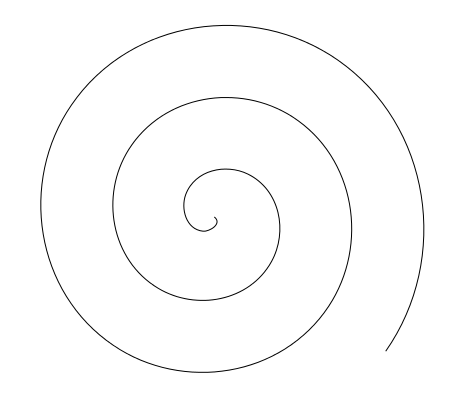
\includegraphics[width=\textwidth]{figures/pic01}
  \caption{Как страшно жить}
  \label{fig:spire01}
\end{figure}


%%% Local Variables:
%%% mode: latex
%%% TeX-master: "rpz"
%%% End:


\backmatter %% Здесь заканчивается нумерованная часть документа и начинаются ссылки и
            %% заключение

\Conclusion



% % Список литературы при помощи BibTeX
% Юзать так:
%
% pdflatex rpz
% bibtex rpz
% pdflatex rpz

\bibliographystyle{gost780u}
\bibliography{rpz}

%%% Local Variables: 
%%% mode: latex
%%% TeX-master: "rpz"
%%% End: 


\appendix   % Тут идут приложения

\chapter{Картинки}
\label{cha:appendix1}

\begin{figure}
\centering
\caption{Картинка в приложении. Страшная и ужасная.}
\end{figure}

%%% Local Variables: 
%%% mode: latex
%%% TeX-master: "rpz"
%%% End: 

% \chapter{Еще картинки}
\label{cha:appendix2}

\begin{figure}
\centering
\caption{Еще одна картинка, ничем не лучше предыдущей. Но надо же как-то заполнить место.}
\end{figure}

%%% Local Variables: 
%%% mode: latex
%%% TeX-master: "rpz"
%%% End: 


\end{document}

%%% Local Variables:
%%% mode: latex
%%% TeX-master: t
%%% End:
